% ============================================================
% CHAPTER 3 -- ANALYSIS / SOFTWARE REQUIREMENTS SPECIFICATION
% FEMCARE: An AI-Powered Women's Reproductive Health Platform
% ============================================================

\chapter{Analysis / Software Requirements Specification (SRS)}\doublespacing
\label{chap:srs}

% ------------------------------------------------------------
\section{Introduction}
\label{sec:srs-intro}

This chapter documents the system analysis and software requirements for FEMCARE. It identifies the limitations of existing systems that FEMCARE is designed to address, establishes the user requirements derived from the intended application, and specifies the functional and non-functional requirements that governed the system's development. The feasibility and constraints of the project are also considered. Architectural design, implementation details, and testing procedures are covered in subsequent chapters.

% ------------------------------------------------------------
\section{Existing System and its Limitations}
\label{sec:existing}

Current digital tools for women's reproductive health fall broadly into two categories: cycle-tracking applications and general-purpose health information services. While cycle-tracking applications allow users to record period dates and flow intensity, they provide no structured clinical risk screening, and their outputs are limited to predicted period dates and general cycle statistics. \cite{epstein2017}\cite{li2021} A user whose logs indicate patterns associated with PCOS -- such as irregular cycles, excess facial hair, or skipped periods -- receives no risk indication from such tools. \cite{zad2024}\cite{ahmed2023}

General-purpose AI assistants are not restricted to women's health and cannot tailor responses to a user's personal health history. \cite{kim2024} Appointment booking for women's health consultations in cities such as Vadodara typically requires telephone contact or direct walk-in visits. No unified digital platform currently provides cycle tracking, structured PCOS risk screening, scoped health guidance, and local provider booking in a single authenticated application. The key limitations motivating FEMCARE are summarised in Table~\ref{tab:existing-limitations}.

\begin{table}[h!]
\centering
\caption{Limitations of Existing Systems and How FEMCARE Addresses Them}
\label{tab:existing-limitations}
\renewcommand{\arraystretch}{1.4}
\begin{tabular}{|p{4.2cm}|p{8.1cm}|}
\hline
\rowcolor[HTML]{D9D9D9}
\textbf{Limitation of Existing Systems} & \textbf{Description} \\
\hline
No integrated PCOS assessment &
Existing cycle-tracking applications primarily record menstrual data but do not provide a structured assessment based on relevant health and clinical inputs. FEMCARE provides an 18-feature assessment that evaluates the entered parameters and returns a PCOS risk result with a confidence measure. \\
\hline
No domain-restricted AI health assistance &
General-purpose AI assistants are not constrained to women's reproductive health and cannot personalise responses using the user's own health data. FEMCARE provides an AI assistant restricted to this domain, enriched with the authenticated user's real cycle and symptom information. \\
\hline
No digital appointment booking for local providers &
Booking a women's health consultation in cities such as Vadodara typically requires telephone contact or walk-in visits. FEMCARE provides online slot booking for ten local providers with automated confirmation and cancellation emails. \\
\hline
No integrated reproductive health awareness &
Health information on conditions such as endometriosis, fibroids, and cervical health is not integrated within existing tracking tools. FEMCARE includes a searchable awareness module covering eight reproductive health conditions, warning signs, and prevention guidance. \\
\hline
Absence of database-level user data isolation &
Lightweight tracking applications often store data locally or rely on application-layer filtering without enforcing per-user access controls at the database level. FEMCARE applies Row Level Security policies in PostgreSQL, ensuring that each user can access only their own data. \\
\hline
\end{tabular}
\end{table}

% ------------------------------------------------------------
\section{Proposed System Overview}
\label{sec:proposed}

FEMCARE is proposed as an authenticated, cloud-backed web application that integrates menstrual cycle tracking, an 18-feature PCOS risk assessment module, a topic-restricted AI health assistant, healthcare provider discovery and booking, and educational health awareness content. All user data is stored in a Supabase-managed PostgreSQL database with Row Level Security policies enforced at the database level. The system is designed as a screening and awareness platform and explicitly does not replace professional medical diagnosis or consultation.

% ------------------------------------------------------------
\section{User Requirements}
\label{sec:user-req}

Based on the intended user group and the implemented application, the following user requirements were identified:

\begin{enumerate}
    \item \textbf{Authentication:} Users must be able to register with a name, email address, password, age, average cycle length, and last period date, and subsequently log in and out securely.

    \item \textbf{Cycle and Symptom Logging:} Users must be able to record daily menstrual data including flow type, pain level, mood, and symptoms for any selected date.

    \item \textbf{Dashboard Overview:} Users must be able to view their current cycle day, phase, recent logged health data, and a navigable monthly calendar from a single screen.

    \item \textbf{PCOS Risk Assessment:} Users must be able to complete a guided health assessment that collects clinical indicators and returns a risk classification with a confidence measure.

    \item \textbf{AI Health Guidance:} Users must be able to ask health questions and receive educational responses within the domain of women's reproductive health.

    \item \textbf{Provider Discovery and Booking:} Users must be able to view local healthcare providers on a map, check slot availability, book an appointment, and cancel a booking.

    \item \textbf{Health Awareness:} Users must be able to browse, search, and filter educational content on reproductive health conditions and warning signs.

    \item \textbf{Profile Management:} Users must be able to view and update their profile information including name, email, cycle length, and last period date.

    \item \textbf{Email Notifications:} Users should receive an email confirmation upon booking or cancelling an appointment.
\end{enumerate}

% ------------------------------------------------------------
\section{Functional Requirements}
\label{sec:functional}

The functional requirements of FEMCARE, derived from the implemented application, are specified in Table~\ref{tab:fr}.

\begin{table}[h!]
\centering
\caption{Functional Requirements}
\label{tab:fr}
\renewcommand{\arraystretch}{1.4}
\begin{tabular}{|p{1.2cm}|p{3.5cm}|p{8cm}|}
\hline
\rowcolor[HTML]{D9D9D9}
\textbf{ID} & \textbf{Requirement} & \textbf{Description} \\
\hline
FR-01 & User Registration & The system shall allow new users to register with name, email, password, age, cycle length, and last period date. \\
\hline
FR-02 & User Authentication & The system shall authenticate users via email and password, establish a persistent session, and redirect unauthenticated requests to the login screen. \\
\hline
FR-03 & Profile Management & Authenticated users shall be able to view and update their profile data stored in the database. \\
\hline
FR-04 & Daily Cycle Logging & Users shall be able to log flow, pain level, mood, and symptoms for any selected date. A unique constraint shall prevent duplicate entries per user per date. \\
\hline
FR-05 & Dashboard Display & The dashboard shall display the current cycle day, phase, a monthly calendar with period and fertility highlights, and the most recently logged health data. \\
\hline
FR-06 & PCOS Assessment & The system shall present an 18-question assessment, automatically calculate the LH/FSH ratio from user-entered values, submit data to the backend, and display the returned risk classification and confidence percentage. \\
\hline
FR-07 & ML-Based Prediction & The backend shall process assessment inputs using a pre-trained XGBoost classifier and return a risk level (Low, Moderate, or High Risk). A heuristic fallback shall be used when the model is unavailable. \\
\hline
FR-08 & AI Health Assistant & The system shall provide a chatbot constrained to women's reproductive health topics. Responses shall be rejected for out-of-scope queries and enriched with the user's real health data when authenticated. \\
\hline
FR-09 & Provider Discovery & The system shall display healthcare providers on an interactive map and as a list, showing name, specialty, address, and contact information. \\
\hline
FR-10 & Appointment Booking & Authenticated users shall be able to book from sixteen daily time slots per provider. The system shall prevent confirmed double-bookings for the same provider, date, and slot. \\
\hline
FR-11 & Booking Management & Users shall be able to view their booking history and cancel a confirmed booking. Cancelled slots shall become available for re-booking. \\
\hline
FR-12 & Email Notifications & The system shall send a confirmation email upon successful booking and a cancellation email upon successful cancellation, including booking details and a booking reference. \\
\hline
FR-13 & Health Awareness & The system shall display educational content on eight reproductive health conditions with search and category filter functionality, and a detail view for each condition. \\
\hline
FR-14 & Period and Symptom History & Users shall be able to view historical period records and symptom log entries. \\
\hline
\end{tabular}
\end{table}

% ------------------------------------------------------------
\section{Non-Functional Requirements}
\label{sec:nonfunctional}

The non-functional requirements governing FEMCARE are specified in Table~\ref{tab:nfr}. The security requirements NFR-01 and NFR-02 reflect established best practices for privacy and data protection in mobile health systems. \cite{kotz2016}

\begin{table}[h!]
\centering
\caption{Non-Functional Requirements}
\label{tab:nfr}
\renewcommand{\arraystretch}{1.4}
\begin{tabular}{|p{1.2cm}|p{3cm}|p{8.5cm}|}
\hline
\rowcolor[HTML]{D9D9D9}
\textbf{ID} & \textbf{Category} & \textbf{Requirement} \\
\hline
NFR-01 & Security & All user health data shall be isolated at the database level using Row Level Security policies, ensuring that no user can access another user's records. \\
\hline
NFR-02 & Security & Passwords shall be managed exclusively by Supabase Authentication. No application table shall store plaintext or hashed passwords. API keys and service credentials shall be stored server-side in environment variables only. \\
\hline
NFR-03 & Reliability & Booking creation shall succeed independently of email delivery. If the email notification service is unavailable, the booking shall remain confirmed and the user shall be informed. \\
\hline
NFR-04 & Reliability & The PCOS assessment shall remain operational through a heuristic fallback when the XGBoost model cannot be loaded. \\
\hline
NFR-05 & Reliability & Frontend API calls shall safely handle non-JSON server responses without application crashes. \\
\hline
NFR-06 & Usability & The application shall be responsive and usable on standard desktop and mobile browsers without a native application installation. \\
\hline
NFR-07 & Usability & Empty data states (no cycle logged, no bookings) shall display informative messages rather than blank screens. \\
\hline
NFR-08 & Medical Safety & The AI health assistant shall enforce topic restriction to women's reproductive health and shall direct users to professional medical care for urgent or serious symptoms. \\
\hline
NFR-09 & Maintainability & Awareness content shall be defined in a dedicated data file, separate from UI components, to allow independent updates. \\
\hline
NFR-10 & Availability & The database and authentication layer shall use a managed cloud service (Supabase) to delegate infrastructure availability. \\
\hline
\end{tabular}
\end{table}

% ------------------------------------------------------------
\section{System Constraints}
\label{sec:constraints}

The following constraints are relevant to the current implementation of FEMCARE:

\begin{itemize}
    \item \textbf{External Service Dependency:} The system depends on three cloud services -- Supabase, Groq, and Resend -- for database, LLM inference, and email respectively. Unavailability of these services will affect corresponding functionality.

    \item \textbf{Internet Connectivity:} FEMCARE is a web application with no offline mode. A working internet connection is required to use any feature of the system.

    \item \textbf{Geographic Scope:} The Find Care module currently contains data for ten healthcare providers in Vadodara, Gujarat. No administrative interface exists for adding or modifying provider data without a source code change.

    \item \textbf{PCOS Screening Scope:} The PCOS assessment is a risk screening tool based on user-reported data. It is not a clinical diagnostic instrument and has not been independently clinically validated.

    \item \textbf{Subscription Functionality:} The subscription plans page is a UI comparison only. No payment processing is implemented in the current version.
\end{itemize}

% ------------------------------------------------------------
\section{Hardware and Software Requirements}
\label{sec:hw-sw}

\subsection{Development Requirements}

\begin{table}[h!]
\centering
\caption{Development Environment Requirements}
\label{tab:dev-req}
\renewcommand{\arraystretch}{1.4}
\begin{tabular}{|p{4cm}|p{8.5cm}|}
\hline
\rowcolor[HTML]{D9D9D9}
\textbf{Component} & \textbf{Requirement} \\
\hline
Operating System & Windows 10/11, macOS, or Linux \\
\hline
Node.js & Version 18 or later (for frontend build) \\
\hline
Python & Version 3.11 or later (for backend) \\
\hline
Package Manager & npm (frontend); pip (backend) \\
\hline
Browser & Any modern browser supporting ES2022 modules \\
\hline
Internet Connection & Required for Supabase, Groq API, and Resend API access \\
\hline
\end{tabular}
\end{table}

\subsection{Key Software Dependencies}

\begin{table}[h!]
\centering
\caption{Key Software Dependencies}
\label{tab:sw-deps}
\renewcommand{\arraystretch}{1.4}
\begin{tabular}{|p{3.5cm}|p{3cm}|p{6cm}|}
\hline
\rowcolor[HTML]{D9D9D9}
\textbf{Technology} & \textbf{Layer} & \textbf{Role} \\
\hline
React 18 / Vite 5 & Frontend & UI framework and build tool \\
\hline
Tailwind CSS 3 & Frontend & Utility-first styling \\
\hline
React-Leaflet 4 & Frontend & Interactive provider map \\
\hline
FastAPI / Uvicorn & Backend & REST API server \\
\hline
XGBoost / scikit-learn & Backend & PCOS ML prediction pipeline \\
\hline
Groq SDK & Backend & LLM inference (llama-3.1-8b-instant) \\
\hline
httpx & Backend & Async HTTP client (Resend API calls) \\
\hline
Supabase PostgreSQL & Database & Data persistence and Row Level Security \\
\hline
Supabase Auth & Auth & JWT-based authentication \\
\hline
Resend API & External & Transactional email delivery \\
\hline
\end{tabular}
\end{table}

% ------------------------------------------------------------
\section{Use Case Analysis}
\label{sec:usecases}

\subsection{Actors}

FEMCARE has two actors:

\begin{itemize}
    \item \textbf{Authenticated User:} A registered, logged-in user who can access all protected features of the application.
    \item \textbf{Guest:} An unauthenticated visitor who can access only the Login and Signup pages.
\end{itemize}

\subsection{Use Case Summary}

The major use cases identified for FEMCARE are listed in Table~\ref{tab:usecases}. Figure~\ref{fig:usecase} illustrates the use case diagram of the system.

\begin{figure}[h!]
\centering
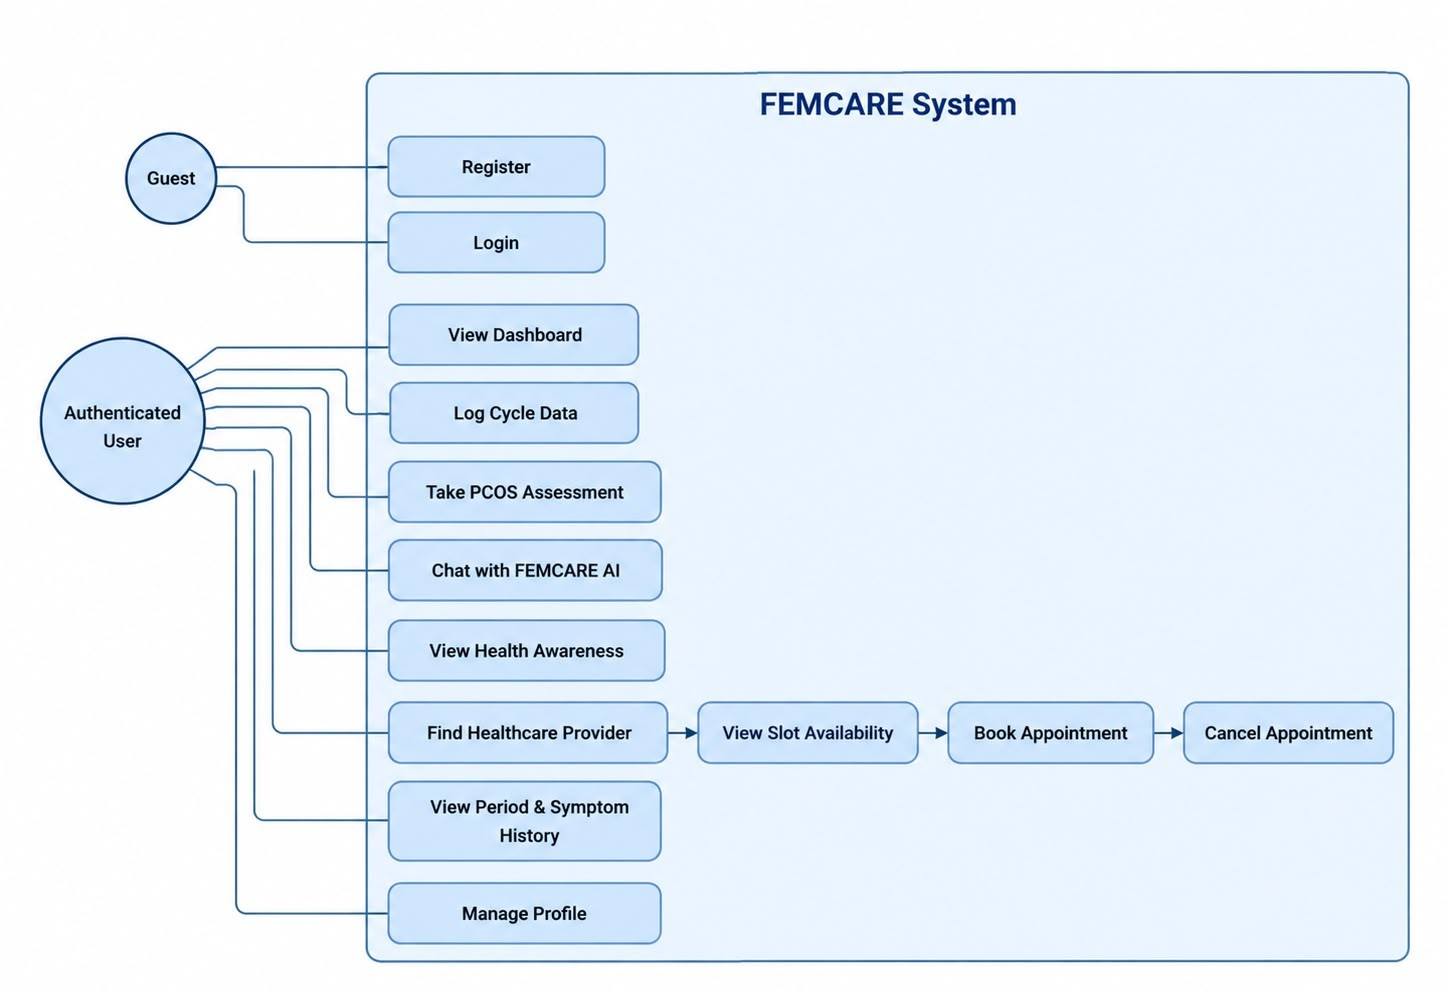
\includegraphics[width=0.85\textwidth]{3.1.jpeg}
\caption{Use Case Diagram of FEMCARE}
\label{fig:usecase}
\end{figure}

\begin{table}[h!]
\centering
\caption{Use Case Summary}
\label{tab:usecases}
\renewcommand{\arraystretch}{1.4}
\begin{tabular}{|p{1.2cm}|p{4cm}|p{2cm}|p{5.5cm}|}
\hline
\rowcolor[HTML]{D9D9D9}
\textbf{UC-ID} & \textbf{Use Case} & \textbf{Actor} & \textbf{Brief Description} \\
\hline
UC-01 & Register & Guest & Create a new account with personal and cycle details. \\
\hline
UC-02 & Login / Logout & Guest / User & Authenticate and manage the user session. \\
\hline
UC-03 & Log Daily Cycle & Auth. User & Record flow, pain, mood, and symptoms for a date. \\
\hline
UC-04 & View Dashboard & Auth. User & View cycle phase, latest logged data, and calendar. \\
\hline
UC-05 & Complete PCOS Assessment & Auth. User & Complete the 18-question quiz and view risk result. \\
\hline
UC-06 & Use AI Health Assistant & Auth. User & Ask reproductive health questions and receive scoped guidance. \\
\hline
UC-07 & Find Healthcare Provider & Auth. User & View providers on the map and in the list. \\
\hline
UC-08 & Book Appointment & Auth. User & Select a provider, date, and slot and confirm booking. \\
\hline
UC-09 & Cancel Appointment & Auth. User & Cancel a confirmed booking. \\
\hline
UC-10 & View Awareness Content & Auth. User & Browse, search, and filter health condition information. \\
\hline
UC-11 & View History & Auth. User & View period and symptom history records. \\
\hline
UC-12 & Update Profile & Auth. User & Edit name, email, cycle length, and last period date. \\
\hline
\end{tabular}
\end{table}

% ------------------------------------------------------------
\section{Feasibility Analysis}
\label{sec:feasibility}

\subsection{Technical Feasibility}

All technologies selected for FEMCARE are mature, actively maintained, and freely available for development use. React and FastAPI are widely adopted frameworks with extensive documentation. Supabase provides managed PostgreSQL with built-in authentication and Row Level Security, removing the need to implement authentication infrastructure from scratch. The Groq API provides low-latency LLM inference, and the Resend API provides a straightforward transactional email service. \cite{maity2025} The XGBoost library is a well-established gradient boosting implementation supported by scikit-learn's pipeline tooling. \cite{ahmed2023}\cite{zad2024} The combination of these services makes the proposed system technically feasible within the scope of a final year project.

\subsection{Operational Feasibility}

The application is a browser-based single-page application requiring no installation. Users interact with familiar interface patterns -- forms, toggles, cards, and maps -- that are consistent with standard web application conventions. The workflow from registration through cycle logging to assessment and booking follows a linear, task-oriented structure that is practical for the intended user group.

\subsection{Economic Feasibility}

The project makes use of free tiers of all external services: Supabase (free tier with 500 MB database and 50,000 monthly active users), Groq API (free tier with generous rate limits for development), and Resend (free tier with 3,000 emails per month). The frontend and backend are developed using open-source frameworks with no licensing costs. The project is therefore economically feasible for development and demonstration purposes at no cost beyond internet access and computing hardware.

% ------------------------------------------------------------

